\documentclass[11pt,a4paper]{article}

\usepackage[utf8]{inputenc}
\usepackage[T1]{fontenc}
\usepackage{lmodern}
\usepackage{geometry}
\usepackage{hyperref}
\usepackage{graphicx}
\usepackage{longtable}
\usepackage{array}
\usepackage{enumitem}
\usepackage{booktabs}
\usepackage{xcolor}
\usepackage{amsmath}
\usepackage{tikz}
\usetikzlibrary{arrows.meta, positioning, shapes.geometric, fit}

\geometry{margin=1in}
\hypersetup{
    colorlinks=true,
    linkcolor=blue,
    urlcolor=blue,
    pdftitle={Problem-to-Paper Research Automation Workflow},
    pdfauthor={Dogukan Ali}
}

\title{Problem-to-Paper: \\ A Gated Agentic Workflow for Automated Research, Planning, Prototyping, and Scientific Drafting}
\author{Dogukan Ali}
\date{\today}

\begin{document}

\maketitle

\begin{abstract}
This document presents a high-level architecture for an automated research assistant system that transforms discovered real-world problems into structured scientific outputs. The workflow begins by gathering candidate problems and trending topics from online sources, then evaluates whether each problem is worth deeper investigation. For the accepted problems, the system performs literature review and web-based evidence collection, decomposes each problem into sub-problems, and assigns specialized agents to investigate each sub-problem in parallel. A main planner then synthesizes these findings into a single execution plan, which is handed to a coding agent for proof-of-concept implementation. The prototype is then validated through testing, compared against existing alternatives, and finally transformed into a scientific paper draft. The goal of the system is to support independent or institutional research by reducing the manual effort required to move from problem discovery to documented experimental output.
\end{abstract}
\section{Introduction}

The growing amount of publicly available information on the internet creates an opportunity for agentic systems that can identify emerging problems, analyze prior work, generate new ideas, implement prototypes, and document results in scientific form. In a university-like research setting, such a system can act as a research assistant that supports students, researchers, or independent developers in quickly exploring promising topics.

The proposed workflow is not limited to a single task such as scraping or literature review. Instead, it connects multiple stages into a full research pipeline. The system starts with problem discovery, filters and evaluates candidate problems, decomposes selected problems into sub-problems, reasons over collected evidence, and finally builds and evaluates a prototype before drafting a paper-like output.

This document describes the architecture, the sequential and parallel phases, the responsibilities of each agent node, and the expected information flow between stages.

\section{Related Work}

Recent work has explored agentic pipelines for research assistance, literature synthesis, code generation, and scientific writing. However, most existing systems focus on only one segment of the workflow, such as literature review, coding assistance, or planning, rather than integrating the full path from problem discovery to validated research output. In this section, we review the most relevant lines of work and position our proposed Problem-to-Paper architecture within them.

\subsection{Automated Literature Review and Research Assistance}

A growing body of work investigates the use of large language models and multi-agent systems for literature review generation and scientific assistance. Recent systems such as LiRA employ multiple specialized agents, including researcher, writer, and reviewer roles, to retrieve papers, summarize evidence, and iteratively improve the readability and reliability of literature reviews \cite{lira2025,reflexion2023}. Similarly, survey and review generation systems such as MASS and AutoSurvey demonstrate that LLM-based pipelines can support reference retrieval, summarization, and structured academic drafting.

These systems represent an important step toward automated research support, but they generally begin with a predefined research topic. In other words, they assume that the problem of interest has already been selected by the user. By contrast, our proposed architecture includes an earlier phase of problem discovery and viability assessment, enabling the system to identify candidate research opportunities directly from web and community signals before literature review begins.

\subsection{Agentic Retrieval and Multi-Agent Research Workflows}

Another relevant area is agentic retrieval-augmented generation. Recent surveys on Agentic RAG describe how autonomous agents can combine planning, tool use, reflection, and retrieval to manage complex multi-step reasoning tasks \cite{agenticrag2025}. These systems improve upon static retrieval pipelines by introducing adaptive query generation, iterative context refinement, and multi-agent coordination.

This line of work is closely related to our design because our system also relies on agents to gather and refine evidence from heterogeneous sources. However, most agentic retrieval systems are designed to improve answering or summarization quality for a given task. They do not typically include explicit problem decomposition, parallel sub-problem planning, or downstream prototype generation. Our architecture extends this paradigm by connecting agentic retrieval to planning, implementation, validation, and final paper drafting.

\subsection{Planning Agents and Task Decomposition}

Explicit planning has become a central idea in modern LLM-based agents. The ReAct framework demonstrated that combining reasoning traces with actions improves task decomposition and tool use \cite{react2023}. Plan-and-Solve prompting further showed that asking models to first devise a plan before execution reduces missing-step errors and improves reasoning quality \cite{planandsolve2023}. More recently, ReWOO formalized a plan-then-execute workflow in which the model first emits a structured plan and then fills evidence placeholders during execution \cite{rewoo2024}.

These approaches strongly motivate the planning layer in our architecture. Rather than sending raw research findings directly to a coding agent, our system introduces a dedicated plan synthesis phase. This phase collects outputs from multiple specialized sub-agents, removes duplication, resolves conflicts, ranks alternatives, and produces a coherent execution plan. In this sense, our work is aligned with planner--executor architectures, but extends them toward end-to-end research automation rather than general problem solving alone.

\subsection{Autonomous Coding Agents}

The emergence of agentic coding tools has made planning-before-execution increasingly common in software generation systems. Claude Code introduces a dedicated plan mode in which the system analyzes a codebase and proposes a multi-step implementation strategy before making changes \cite{claudecode2026}. Qwen Code similarly exposes a planning or thinking mode that generates an implementation plan before applying edits \cite{qwencode2025}. GitHub Copilot's planning agent also follows a staged workflow in which the system researches the task, aligns on the objective, drafts a plan, and refines it before code changes are made \cite{copilotplan2026}. Framework-oriented implementations such as LangChain's plan-and-execute pattern and OpenAI's multi-agent orchestration examples provide reusable abstractions for separating planning from execution and for coordinating parallel specialized agents \cite{langchainplanning2024,openaiparallelagents2025}.

These systems show that explicit planning improves coding reliability, but they remain primarily focused on implementation tasks that are already defined. They do not perform autonomous topic discovery, research viability screening, or paper-oriented synthesis. Our proposed system builds on their planning principles while embedding them into a broader academic workflow that begins before coding and continues after prototype development.

\subsection{Testing, Reflection, and Validation Loops}

Several recent approaches emphasize that generation alone is insufficient without validation. Reflexion introduced self-critique and iterative correction as a means of improving agent reliability \cite{reflexion2023}. In practice, coding workflows increasingly incorporate test-driven or test-assisted generation, where unit tests, execution feedback, and iterative refinement are used to correct errors and stabilize outputs \cite{addyworkflow2026}. These ideas also appear in engineering-oriented agent frameworks, where the execution loop includes code running, observation, error analysis, and re-planning.

Our system adopts this philosophy by treating testing and benchmarking as first-class phases rather than optional post-processing steps. After prototype generation, a validation agent verifies functionality and collects measurable evidence. A separate comparison stage then positions the generated solution against existing methods and baselines. This creates a stronger bridge between implementation and academic evaluation than is usually found in either literature-review agents or coding-only assistants.

\subsection{AI-Assisted Scientific Writing}

AI-supported academic writing has also advanced rapidly, with systems assisting in abstract generation, related work drafting, citation-aware summarization, and even full report generation. Multi-agent writing pipelines show that specialized writer, editor, and reviewer roles can improve coherence and structure in generated academic text \cite{lira2025}. Nonetheless, most current writing systems operate as downstream drafting assistants. They depend on a user or upstream process to provide the topic, evidence, and experimental results.

In contrast, our architecture treats scientific writing as the final stage of a unified workflow. The paper writer agent is not an isolated text generator; it consumes structured outputs from previous phases, including discovered problems, literature findings, synthesized plans, prototype behavior, validation outcomes, and comparative analysis. This allows the final document to reflect the entire reasoning and experimentation chain rather than merely summarizing isolated notes.

\subsection{Research Gap and Positioning of Our Work}

Taken together, prior work provides strong foundations for automated retrieval, reasoning, coding, testing, and writing. However, these capabilities are typically studied in isolation. Literature review agents assume a predefined topic. Planning agents assume a predefined task. Coding agents assume that the problem has already been translated into implementation requirements. Writing agents assume that the underlying research process has already been completed.

Our work addresses this fragmentation by proposing a gated, end-to-end Problem-to-Paper workflow. The key novelty is not a single new agent type, but the integration of multiple stages into one coordinated architecture:
\begin{enumerate}
    \item automated problem discovery from web sources,
    \item research viability assessment,
    \item problem formulation and sub-problem decomposition,
    \item parallel multi-agent research and planning,
    \item centralized plan synthesis,
    \item autonomous solution development,
    \item testing and comparative evaluation, and
    \item AI-assisted scientific drafting.
\end{enumerate}

To the best of our knowledge, existing systems do not combine all of these components into a single research automation pipeline with explicit gating and synthesis. Our proposed architecture therefore contributes a unifying framework that connects problem discovery, planning, prototyping, validation, and academic writing into one reproducible agentic workflow.

\section{Problem Definition and Scope}

The goal of the system is to provide an automated \textbf{Problem-to-Paper} workflow. In other words, the system should:

\begin{enumerate}[label=\arabic*.]
    \item Discover relevant and promising problems from online sources,
    \item Evaluate whether these problems are worth researching,
    \item Collect prior knowledge from literature and web resources,
    \item Decompose accepted problems into manageable sub-problems,
    \item Generate and synthesize solution plans,
    \item Build a proof-of-concept implementation,
    \item Test and validate that implementation,
    \item Compare the proposed approach with existing alternatives,
    \item Draft a scientific paper or research-style report based on the full process.
\end{enumerate}

The workflow is designed to combine research automation, software prototyping, and paper generation into one coordinated architecture.

\section{System Overview}

The overall workflow can be summarized as follows:

\begin{enumerate}[label=\arabic*.]
    \item \textbf{Problem Gathering}: Identify candidate problems, trends, unanswered questions, or open technical needs from online sources.
    \item \textbf{Worth-It Evaluation}: For each candidate problem, determine whether it is sufficiently relevant, feasible, and promising for deeper investigation.
    \item \textbf{Problem Formulation and Decomposition}: Normalize accepted problems into clear research statements and decompose them into sub-problems.
    \item \textbf{Parallel Research Collection}: Launch specialized sub-agents in parallel to gather literature, related work, web evidence, implementation references, and baseline solutions for each sub-problem.
    \item \textbf{Plan Synthesis}: Aggregate the outputs of all sub-agents and synthesize them into a single coherent solution plan.
    \item \textbf{Prototype Planning and Coding}: Convert the chosen plan into a coding roadmap and implement a proof-of-concept.
    \item \textbf{Testing and Validation}: Execute tests to verify that the prototype functions correctly and produces meaningful results.
    \item \textbf{Comparison and Evaluation}: Compare the resulting solution against prior work, known alternatives, or baseline approaches.
    \item \textbf{Paper Drafting and Conclusion}: Produce a structured scientific draft including motivation, related work, method, implementation, experiments, results, comparison, discussion, and conclusion.
\end{enumerate}

\begin{figure}[t]
\centering
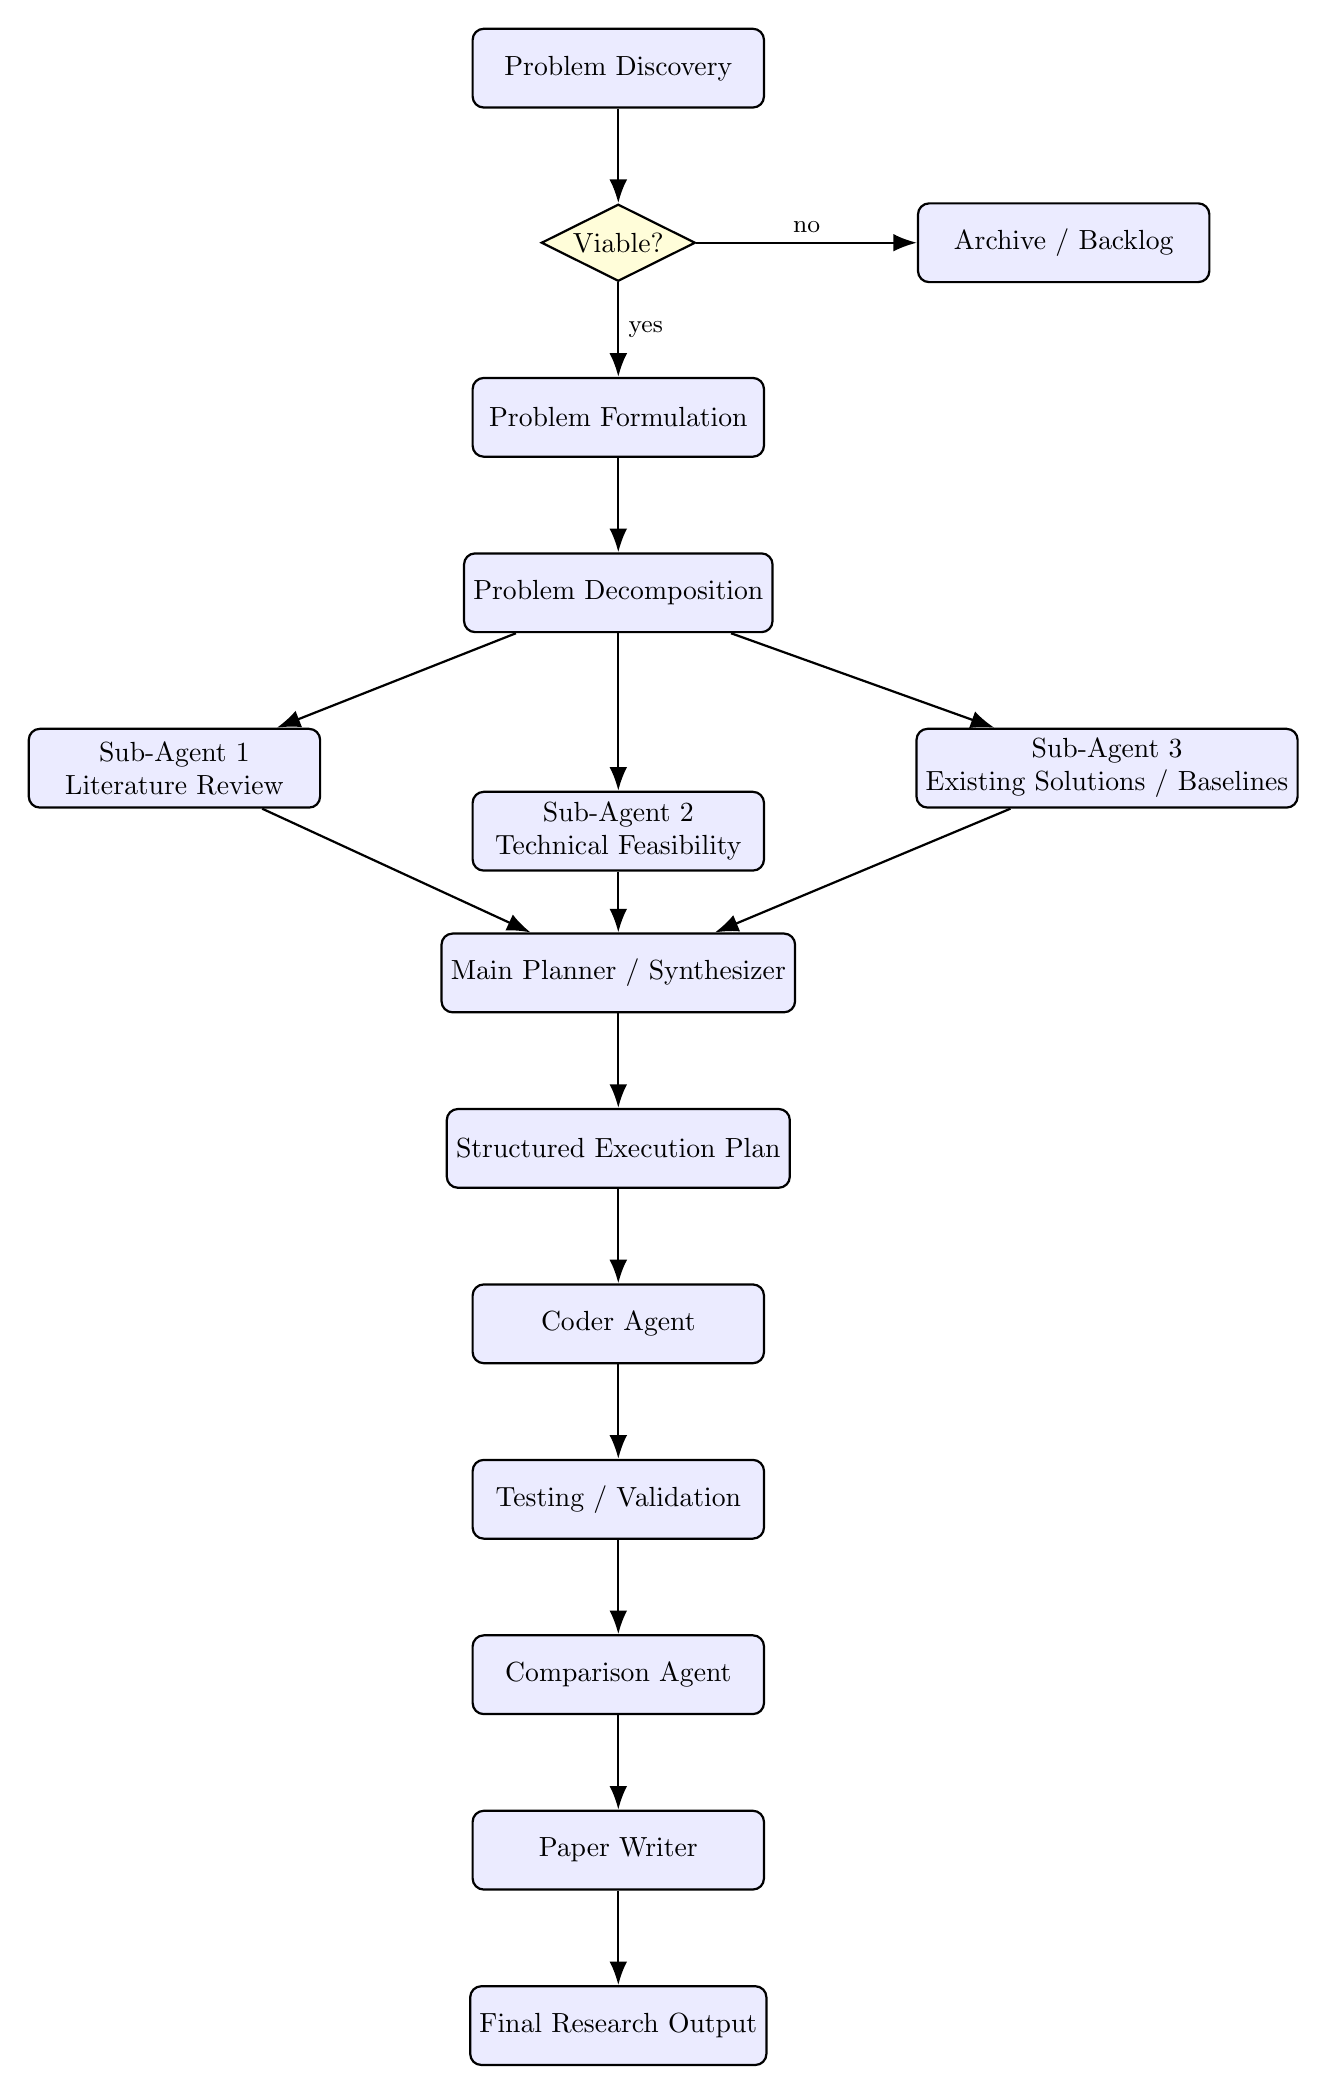
\begin{tikzpicture}[
    node distance=1.2cm and 1.4cm,
    block/.style={
        rectangle,
        rounded corners,
        draw=black,
        thick,
        align=center,
        minimum width=3.7cm,
        minimum height=1cm,
        fill=blue!8
    },
    decision/.style={
        diamond,
        draw=black,
        thick,
        align=center,
        aspect=2,
        fill=yellow!15,
        inner sep=1.5pt
    },
    arrow/.style={-{Latex[length=3mm]}, thick}
]

\node[block] (discover) {Problem Discovery};
\node[decision, below=of discover] (viability) {Viable?};

\node[block, right=2.8cm of viability] (archive) {Archive / Backlog};

\node[block, below=of viability] (formulate) {Problem Formulation};
\node[block, below=of formulate] (decompose) {Problem Decomposition};

\node[block, below left=1.2cm and 1.8cm of decompose] (lit) {Sub-Agent 1\\Literature Review};
\node[block, below=2.0cm of decompose] (tech) {Sub-Agent 2\\Technical Feasibility};
\node[block, below right=1.2cm and 1.8cm of decompose] (baseline) {Sub-Agent 3\\Existing Solutions / Baselines};

\node[block, below=3.8cm of decompose] (synth) {Main Planner / Synthesizer};
\node[block, below=of synth] (plan) {Structured Execution Plan};
\node[block, below=of plan] (coder) {Coder Agent};
\node[block, below=of coder] (test) {Testing / Validation};
\node[block, below=of test] (compare) {Comparison Agent};
\node[block, below=of compare] (writer) {Paper Writer};
\node[block, below=of writer] (output) {Final Research Output};

\draw[arrow] (discover) -- (viability);
\draw[arrow] (viability) -- node[right] {\small yes} (formulate);
\draw[arrow] (viability) -- node[above] {\small no} (archive);

\draw[arrow] (formulate) -- (decompose);

\draw[arrow] (decompose) -- (lit);
\draw[arrow] (decompose) -- (tech);
\draw[arrow] (decompose) -- (baseline);

\draw[arrow] (lit) -- (synth);
\draw[arrow] (tech) -- (synth);
\draw[arrow] (baseline) -- (synth);

\draw[arrow] (synth) -- (plan);
\draw[arrow] (plan) -- (coder);
\draw[arrow] (coder) -- (test);
\draw[arrow] (test) -- (compare);
\draw[arrow] (compare) -- (writer);
\draw[arrow] (writer) -- (output);

\end{tikzpicture}
\caption{High-level workflow graph of the proposed Problem-to-Paper pipeline.}
\label{fig:workflow_graph}
\end{figure}

Figure~\ref{fig:workflow_graph} summarizes the end-to-end control flow of the proposed system, from problem discovery and viability assessment to implementation, evaluation, and final research output.

\section{Architecture}
\label{sec:architecture}

This section presents the architectural design of the proposed \emph{Problem-to-Paper} system. The overall goal of the architecture is to transform weakly structured online signals into a validated research artifact through a sequence of coordinated agentic stages. Rather than treating research, planning, implementation, and writing as separate workflows, the system connects them into a single gated pipeline. This design allows the framework to move from candidate problem discovery to paper drafting while preserving explicit control over filtering, decomposition, execution, and evaluation.

Figure~\ref{fig:architecture} illustrates the high-level architecture. The workflow begins with a \emph{Problem Gathering Agent}, which scans external sources and identifies candidate topics, research opportunities, or unresolved practical problems. Since not every discovered topic justifies full downstream processing, the output of this stage is passed to a decision node labeled \emph{Worth-it?}. This node acts as a research viability gate: low-value or weakly motivated topics are rejected and archived, while promising topics continue into the main pipeline.

\begin{figure}[t]
\centering
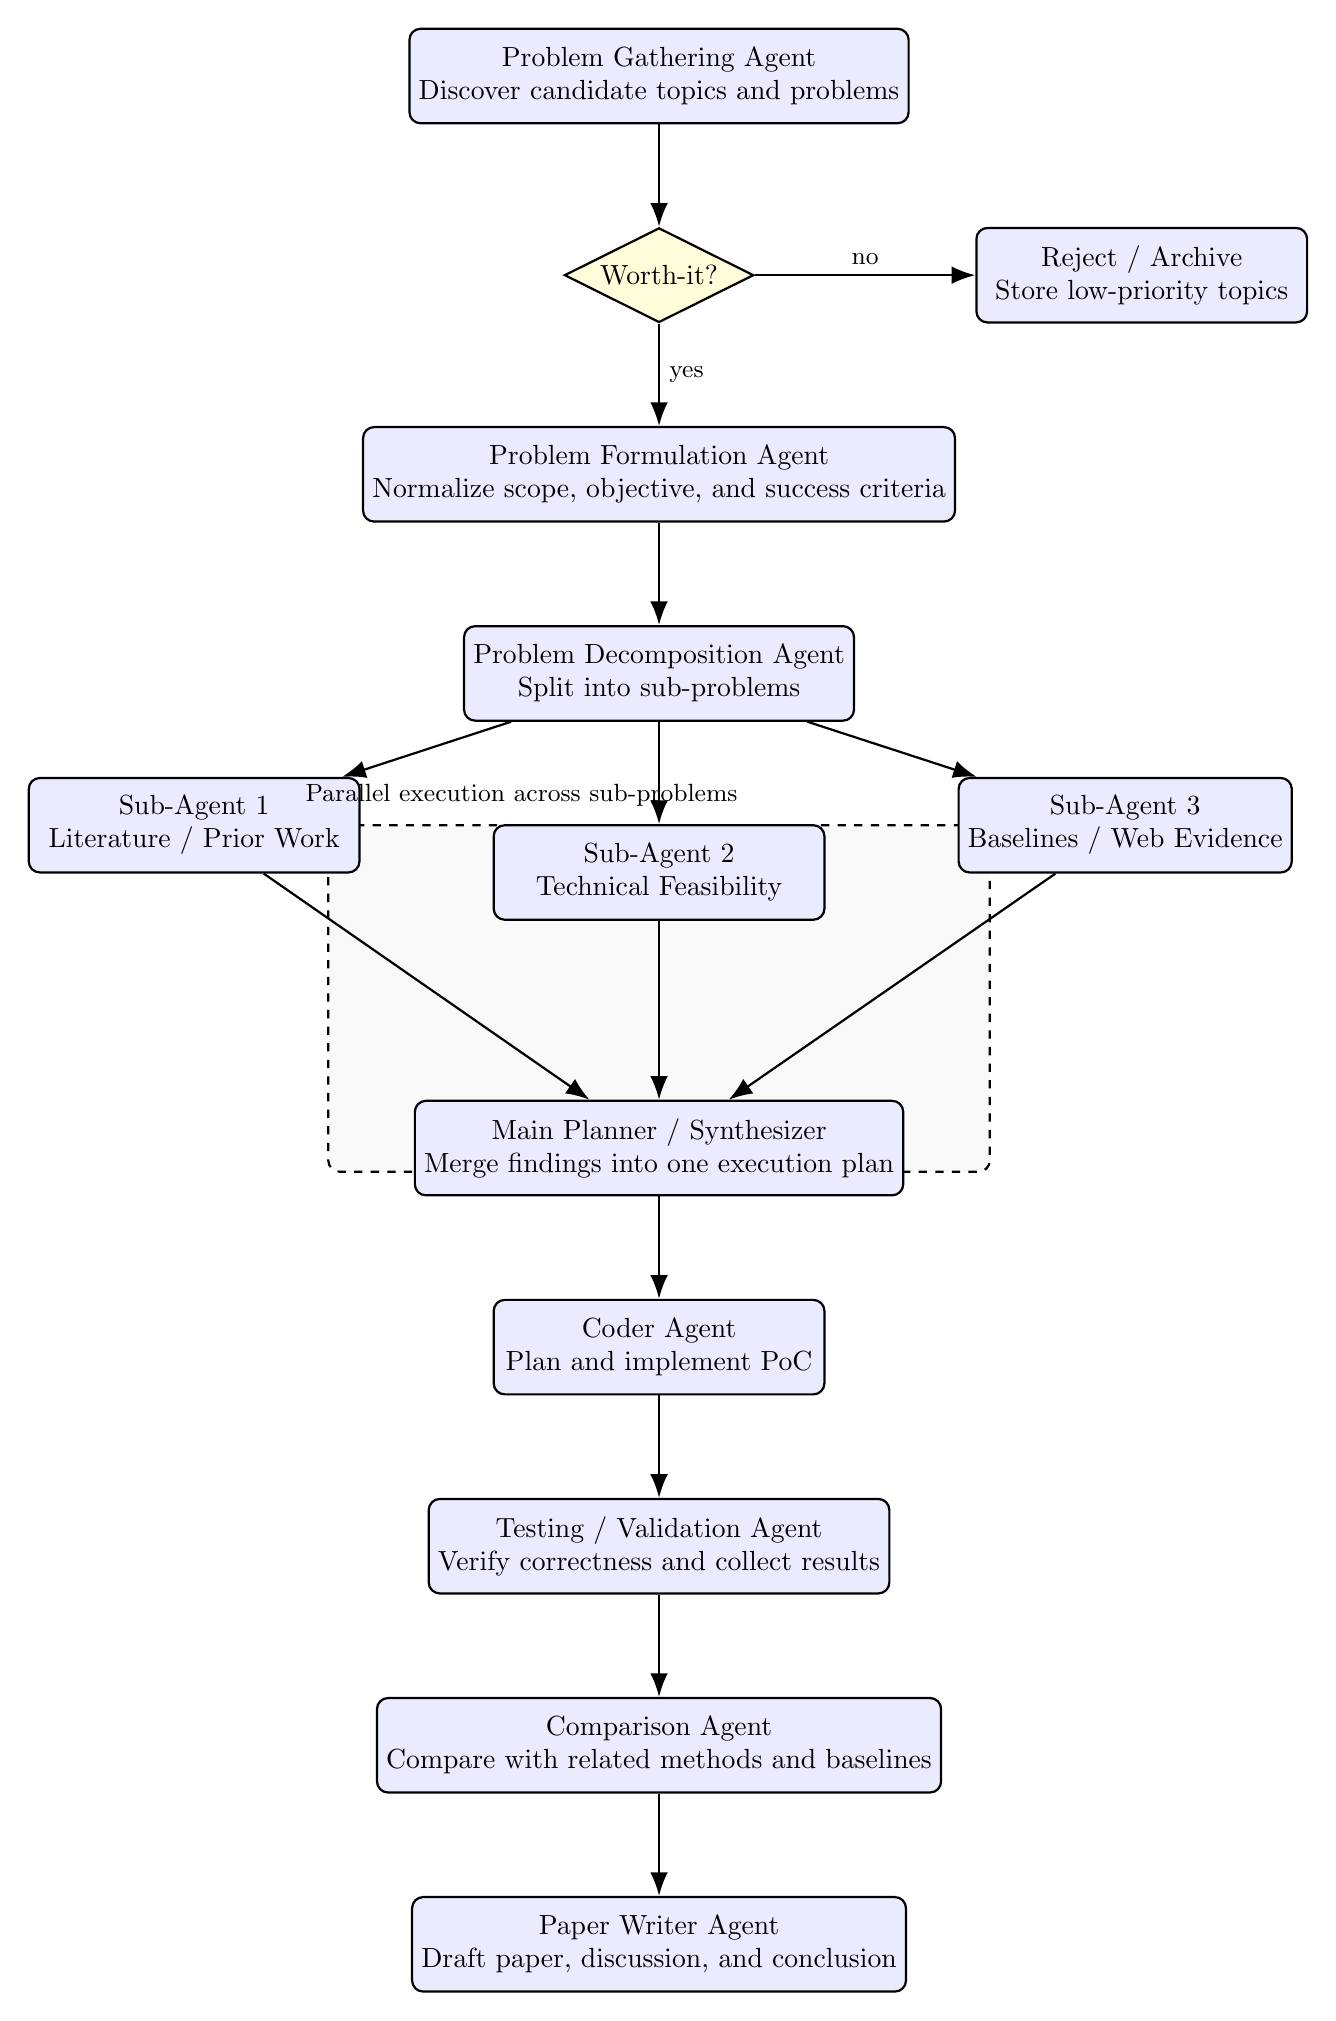
\begin{tikzpicture}[
    node distance=1.3cm and 1.6cm,
    agent/.style={
        rectangle,
        rounded corners,
        draw=black,
        thick,
        align=center,
        minimum width=4.2cm,
        minimum height=1.2cm,
        fill=blue!8
    },
    decision/.style={
        diamond,
        draw=black,
        thick,
        align=center,
        aspect=2,
        fill=yellow!15,
        inner sep=2pt
    },
    parallel/.style={
        rectangle,
        rounded corners,
        draw=black,
        dashed,
        thick,
        align=center,
        minimum width=8.4cm,
        minimum height=4.4cm,
        fill=gray!5
    },
    arrow/.style={-{Latex[length=3mm]}, thick}
]

\node[agent] (problem) {Problem Gathering Agent\\Discover candidate topics and problems};

\node[decision, below=of problem] (gate) {Worth-it?};

\node[agent, right=2.8cm of gate] (archive) {Reject / Archive\\Store low-priority topics};

\node[agent, below=of gate] (formulation) {Problem Formulation Agent\\Normalize scope, objective, and success criteria};

\node[agent, below=of formulation] (decomposition) {Problem Decomposition Agent\\Split into sub-problems};

\node[parallel, below=of decomposition] (parallelbox) {};

\node[agent, below left=0.7cm and 1.3cm of decomposition] (sub1) {Sub-Agent 1\\Literature / Prior Work};
\node[agent, below=of decomposition] (sub2) {Sub-Agent 2\\Technical Feasibility};
\node[agent, below right=0.7cm and 1.3cm of decomposition] (sub3) {Sub-Agent 3\\Baselines / Web Evidence};

\node[agent, below=4.8cm of decomposition] (planner) {Main Planner / Synthesizer\\Merge findings into one execution plan};

\node[agent, below=of planner] (coder) {Coder Agent\\Plan and implement PoC};

\node[agent, below=of coder] (tester) {Testing / Validation Agent\\Verify correctness and collect results};

\node[agent, below=of tester] (comparator) {Comparison Agent\\Compare with related methods and baselines};

\node[agent, below=of comparator] (writer) {Paper Writer Agent\\Draft paper, discussion, and conclusion};

\draw[arrow] (problem) -- (gate);
\draw[arrow] (gate) -- node[right] {\small yes} (formulation);
\draw[arrow] (gate) -- node[above] {\small no} (archive);

\draw[arrow] (formulation) -- (decomposition);

\draw[arrow] (decomposition) -- (sub1);
\draw[arrow] (decomposition) -- (sub2);
\draw[arrow] (decomposition) -- (sub3);

\draw[arrow] (sub1) -- (planner);
\draw[arrow] (sub2) -- (planner);
\draw[arrow] (sub3) -- (planner);

\draw[arrow] (planner) -- (coder);
\draw[arrow] (coder) -- (tester);
\draw[arrow] (tester) -- (comparator);
\draw[arrow] (comparator) -- (writer);

\node[above right=0.1cm and -0.4cm of parallelbox.north west, align=left] {\small Parallel execution across sub-problems};

\end{tikzpicture}
\caption{High-level gated agentic architecture for the proposed Problem-to-Paper workflow.}
\label{fig:architecture}
\end{figure}

For the problems that pass the viability gate, the next stage is handled by the \emph{Problem Formulation Agent}. This component converts noisy or informal topic descriptions into a more structured representation by clarifying the scope of the problem, the objective of the investigation, and the initial success criteria. This normalization step is important because downstream reasoning quality depends heavily on whether the system works with a precise research statement rather than an ambiguous topic description.

After formulation, the \emph{Problem Decomposition Agent} breaks the accepted problem into smaller and more manageable sub-problems. As shown in Figure~\ref{fig:architecture}, these sub-problems are then assigned to parallel specialized sub-agents. In the present architecture, three representative branches are shown: one focused on \emph{literature and prior work}, one focused on \emph{technical feasibility}, and one focused on \emph{baselines and web evidence}. This fan-out structure is one of the core design decisions of the system. Instead of forcing a single agent to reason about all dimensions of the problem at once, the architecture distributes the analysis across multiple focused branches, thereby improving modularity, interpretability, and scalability.

The outputs of these parallel branches are collected by the \emph{Main Planner / Synthesizer}. This node plays a central role in the architecture. Its function is not merely to aggregate raw findings, but to transform them into a coherent execution strategy. Concretely, the planner is responsible for merging overlapping findings, resolving conflicting recommendations, selecting the most suitable direction among alternatives, and producing a structured plan that can guide implementation. In this sense, the planner acts as the transition point between open-ended research and concrete execution.

Once a plan has been synthesized, the workflow proceeds to the \emph{Coder Agent}, which produces a proof-of-concept implementation. The architecture intentionally places coding only after the synthesis phase. This ordering ensures that implementation is guided by a selected strategy rather than by unstructured research output. The result is a more controlled and reproducible transition from idea generation to prototype construction.

The prototype is then passed to the \emph{Testing / Validation Agent}, which checks whether the implementation is executable, whether it behaves as intended, and whether it produces outputs that can support subsequent analysis. This validation stage is followed by the \emph{Comparison Agent}, which positions the generated solution against existing methods, baselines, or related systems. The purpose of this stage is to convert implementation results into comparative evidence that can support academic argumentation.

Finally, the validated and compared output is transferred to the \emph{Paper Writer Agent}. As indicated in Figure~\ref{fig:architecture}, this final stage is responsible for drafting the research narrative, including discussion and conclusion. Unlike a standalone writing assistant, this component operates on the structured artifacts produced by the preceding stages, allowing the final paper draft to reflect the entire reasoning and experimentation pipeline.

Overall, the architecture shown in Figure~\ref{fig:architecture} embodies three key principles. First, it is \emph{gated}, meaning that not every discovered topic proceeds to expensive downstream stages. Second, it is \emph{decompositional}, meaning that accepted problems are split into smaller analytical dimensions handled by specialized agents. Third, it is \emph{progressive}, meaning that the workflow moves from discovery to reasoning, from reasoning to implementation, and from implementation to scientific communication in a structured sequence. These properties make the architecture well suited for an end-to-end research automation setting in which discovery, planning, prototyping, evaluation, and writing must be tightly coordinated.

\section{Methodology}

\subsection{Problem Discovery}

The first phase is responsible for collecting potential research problems. This stage acts as the entry point of the whole workflow. Its objective is not yet to solve a problem, but to identify candidate directions worth investigating.

Possible inputs to this stage may include online discussions, technical forums, research trends, social platforms, developer communities, issue trackers, domain-specific websites, and general web content. The output of this phase is a set of candidate problems or research questions that appear promising, relevant, or insufficiently solved.

The main responsibilities of this phase are:
\begin{itemize}
    \item Identify emerging or important topics,
    \item Filter noisy or low-value signals,
    \item Produce a list of structured problem candidates,
    \item Forward those candidates to the evaluation stage.
\end{itemize}

\subsection{Research Viability Assessment}

Not every discovered problem deserves a full research pipeline. Therefore, the second phase acts as a gatekeeper.

For each candidate problem, an evaluator agent determines whether the topic is worth deeper investigation. This decision may consider:
\begin{itemize}
    \item Relevance and practical importance,
    \item Availability of sufficient literature or evidence,
    \item Novelty or lack of satisfactory existing solutions,
    \item Feasibility of building a proof-of-concept,
    \item Possibility of designing a meaningful evaluation.
\end{itemize}

Problems that do not pass this filter can be archived for future review, while accepted problems continue to the next stages. This gating phase prevents the system from wasting resources on weak or low-impact topics.

\subsection{Problem Formulation}

Accepted problems should not be passed forward in raw form. Before decomposition, the problem should be normalized into a clearer research statement.

This phase is responsible for:
\begin{itemize}
    \item Defining the problem scope,
    \item Clarifying the objective,
    \item Establishing initial success criteria,
    \item Translating informal problem descriptions into structured research questions.
\end{itemize}

This step improves downstream planning quality because sub-agents work better on a precise problem statement than on vague or noisy input.

\subsection{Problem Decomposition}

Once a problem has been properly formulated, the next step is to divide it into manageable sub-problems.

Instead of assigning one large agent to solve everything at once, the system splits the problem into specialized research dimensions such as:
\begin{itemize}
    \item Literature and prior academic work,
    \item Technical feasibility,
    \item Existing tools, baselines, and practical solutions,
    \item Evaluation strategies,
    \item Possible implementation directions.
\end{itemize}

The purpose of this phase is to reduce complexity and improve reasoning quality by creating focused investigative branches.

\subsection{Parallel Evidence Collection}

Each sub-problem is assigned to a specialized sub-agent that works in parallel with the others. This is the main evidence-gathering stage of the workflow.

For each sub-problem, the corresponding agent may gather:
\begin{itemize}
    \item Related literature,
    \item Online technical discussions,
    \item Existing solutions and products,
    \item Blog posts, repositories, or implementation references,
    \item Baseline methods and competing alternatives.
\end{itemize}

This phase may combine structured literature search with unstructured web scraping. The intention is to collect both academic and practical information. Academic literature helps understand the prior state of research, while general web data helps identify practical solutions, common pain points, and implementation patterns.

Because this phase runs per sub-problem, it is naturally suited to parallel execution. This improves scalability and allows the system to explore multiple dimensions of the problem simultaneously.

\subsection{Plan Synthesis}

After the sub-agents complete their work, their outputs are gathered by a main planner or synthesizer. This phase is one of the most important components of the entire architecture.

Its responsibility is not merely to concatenate the sub-agent outputs. Instead, it must:
\begin{itemize}
    \item Remove duplicated findings,
    \item Resolve conflicting recommendations,
    \item Rank alternative approaches,
    \item Select the most suitable solution direction,
    \item Define an execution order,
    \item Produce a single coherent implementation plan,
    \item Establish success and validation criteria for coding.
\end{itemize}

This phase transforms evidence into an actionable plan. The resulting output should be sufficiently structured so that the coding agent can operate without reading all raw research materials.

\subsection{Prototype Development}

Once the planner produces a clear direction, the next step is implementation. The coder agent receives the synthesized solution plan and translates it into an actionable proof-of-concept.

This phase includes:
\begin{itemize}
    \item Breaking down the plan into implementable components,
    \item Selecting a suitable technical stack,
    \item Planning algorithms or modules,
    \item Writing prototype code,
    \item Iteratively improving the implementation.
\end{itemize}

The purpose here is not necessarily to create a production system, but to produce a working prototype that can demonstrate the feasibility of the proposed method.

\subsection{Testing and Validation}

A research idea becomes more convincing when it is validated. Therefore, after implementation, the system enters a testing phase.

The testing and validation agent checks whether:
\begin{itemize}
    \item The code executes successfully,
    \item The prototype behaves as intended,
    \item The output is meaningful,
    \item Basic performance or correctness requirements are met,
    \item The implementation can support claims made in the paper.
\end{itemize}

This stage may include unit-style checks, functional testing, benchmark tasks, or domain-specific evaluation depending on the type of prototype.

\subsection{Comparative Evaluation}

After obtaining test results, the system compares the proposed solution to known alternatives. This comparison stage is essential for positioning the work in relation to prior art.

The comparison agent examines:
\begin{itemize}
    \item Existing methods from literature,
    \item Common practical approaches found online,
    \item Similar tools, systems, or baselines,
    \item Strengths and weaknesses of the new prototype.
\end{itemize}

The goal is to determine where the proposed approach offers improvement, where it performs similarly, and where it may still be weaker. This phase forms the basis of the evaluation and discussion sections of the final paper.

\subsection{Scientific Drafting}

The final phase generates a scientific draft or paper-like output. This stage takes all prior artifacts and organizes them into a readable and structured document.

A typical output may include:
\begin{itemize}
    \item Title and abstract,
    \item Introduction and motivation,
    \item Related work / literature review,
    \item Methodology,
    \item System architecture,
    \item Implementation details,
    \item Experimental setup and testing,
    \item Results and comparison,
    \item Discussion,
    \item Conclusion and future work.
\end{itemize}

This phase does not only summarize the work. It also transforms intermediate artifacts into a presentation suitable for academic communication, project reporting, or independent publication.

\subsection{Planning Logic and Agentic Coordination}

A central design decision in this workflow is that coding must not start immediately after information retrieval. Instead, the system introduces an explicit planning layer.

This design is motivated by the observation that large or complex tasks are handled more effectively when the system first:
\begin{itemize}
    \item gathers evidence,
    \item decomposes the task into smaller components,
    \item reasons over alternatives,
    \item synthesizes a structured plan,
    \item and only then executes implementation.
\end{itemize}

\begin{figure}[t]
\centering
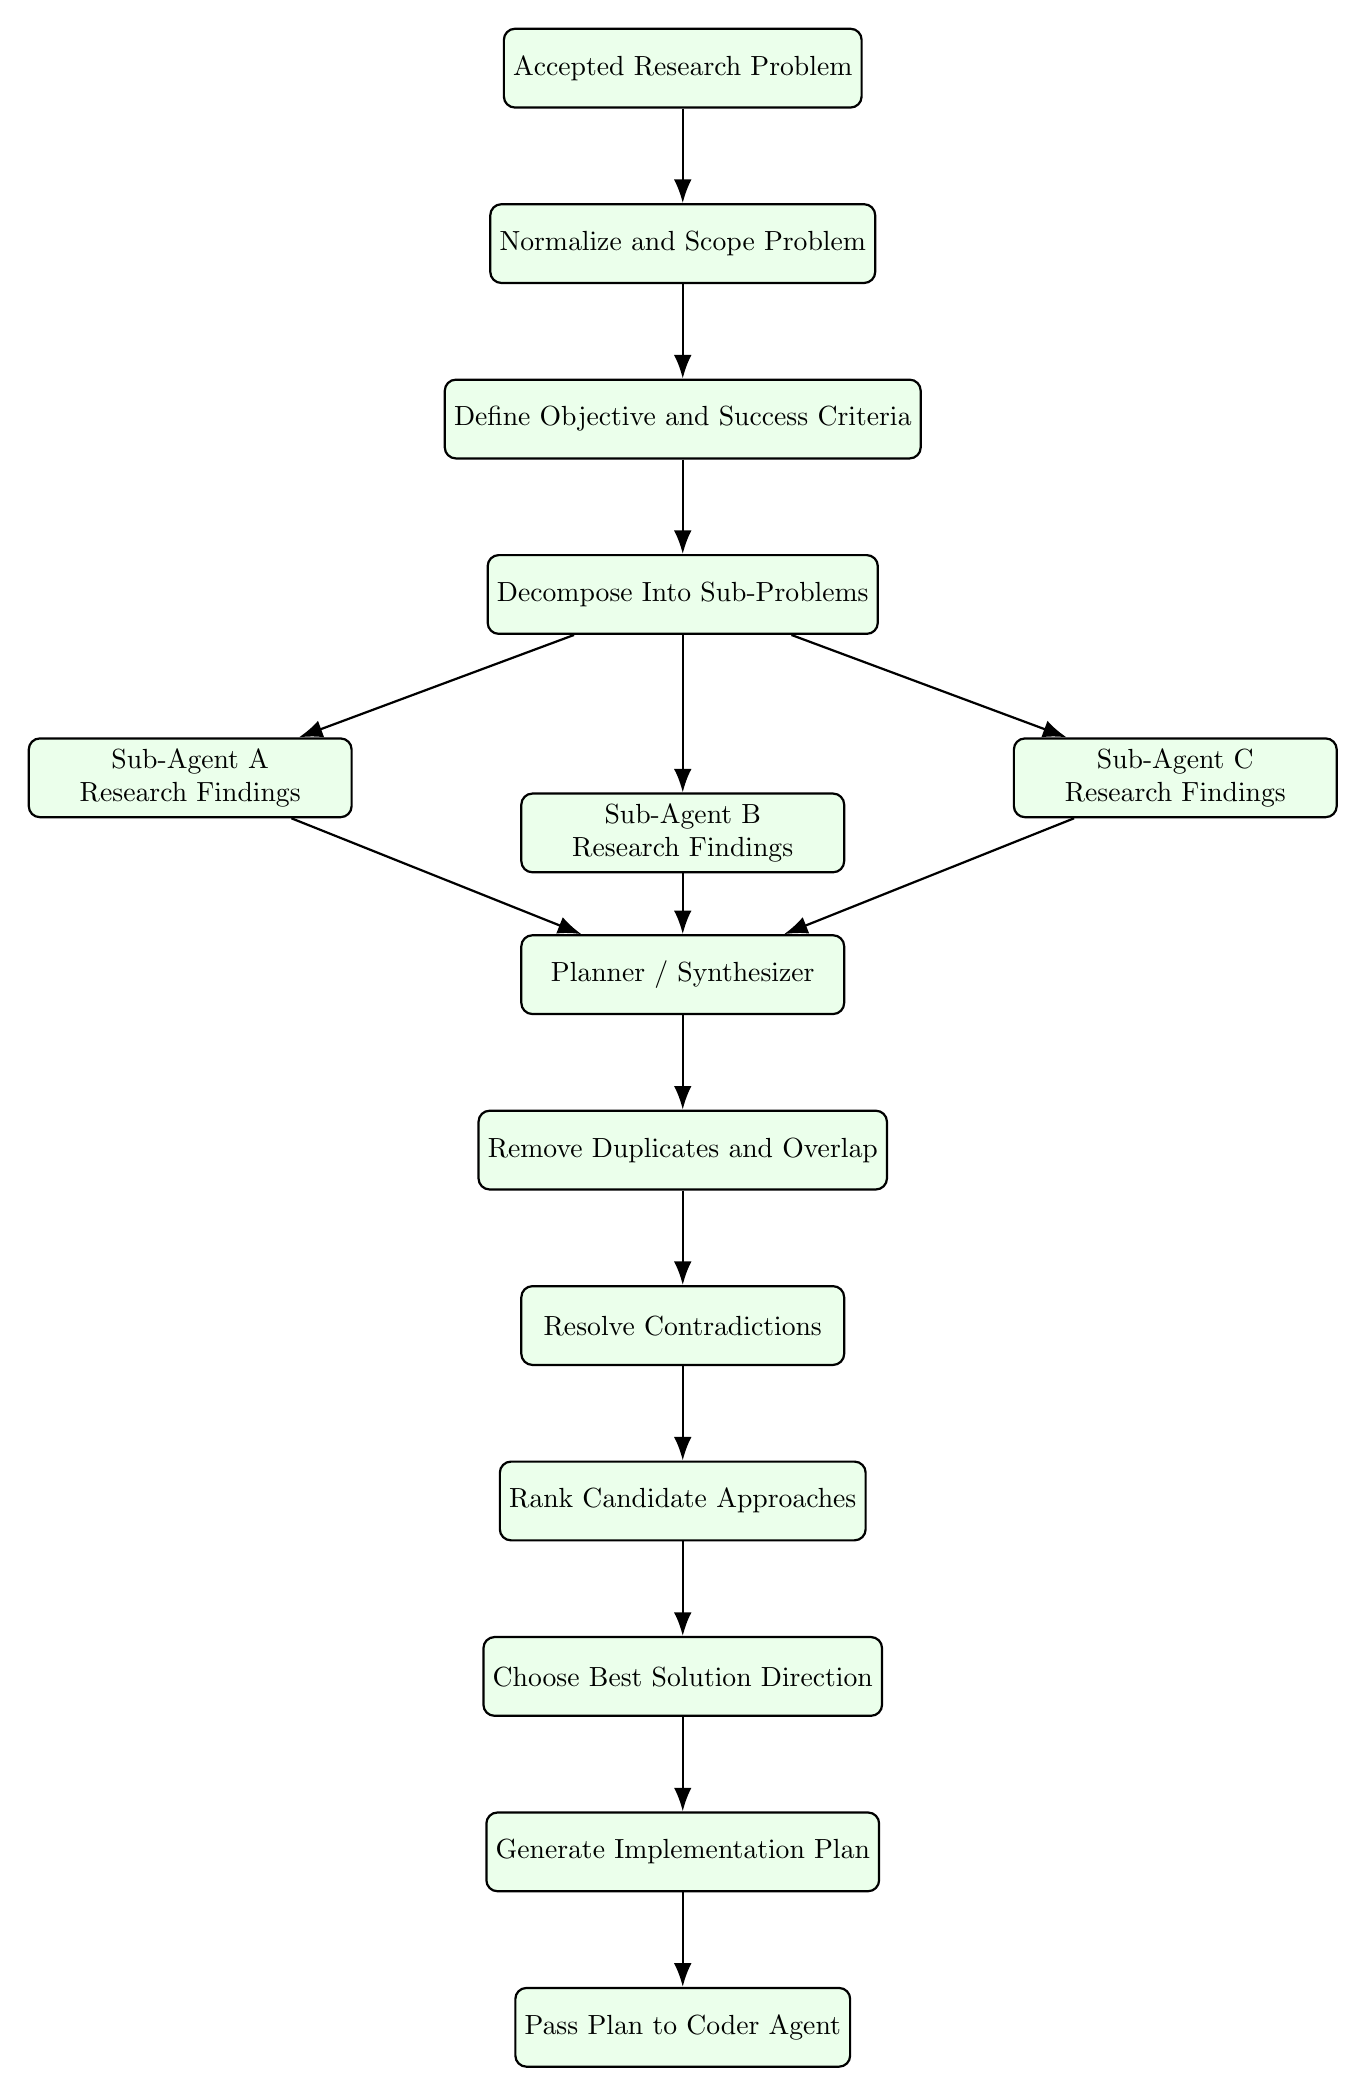
\begin{tikzpicture}[
    node distance=1.2cm and 1.3cm,
    block/.style={
        rectangle,
        rounded corners,
        draw=black,
        thick,
        align=center,
        minimum width=4.1cm,
        minimum height=1cm,
        fill=green!8
    },
    arrow/.style={-{Latex[length=3mm]}, thick}
]

\node[block] (accepted) {Accepted Research Problem};
\node[block, below=of accepted] (normalize) {Normalize and Scope Problem};
\node[block, below=of normalize] (metrics) {Define Objective and Success Criteria};
\node[block, below=of metrics] (split) {Decompose Into Sub-Problems};

\node[block, below left=1.3cm and 1.7cm of split] (suba) {Sub-Agent A\\Research Findings};
\node[block, below=2.0cm of split] (subb) {Sub-Agent B\\Research Findings};
\node[block, below right=1.3cm and 1.7cm of split] (subc) {Sub-Agent C\\Research Findings};

\node[block, below=3.8cm of split] (planner) {Planner / Synthesizer};
\node[block, below=of planner] (dedup) {Remove Duplicates and Overlap};
\node[block, below=of dedup] (resolve) {Resolve Contradictions};
\node[block, below=of resolve] (rank) {Rank Candidate Approaches};
\node[block, below=of rank] (choose) {Choose Best Solution Direction};
\node[block, below=of choose] (impl) {Generate Implementation Plan};
\node[block, below=of impl] (handoff) {Pass Plan to Coder Agent};

\draw[arrow] (accepted) -- (normalize);
\draw[arrow] (normalize) -- (metrics);
\draw[arrow] (metrics) -- (split);

\draw[arrow] (split) -- (suba);
\draw[arrow] (split) -- (subb);
\draw[arrow] (split) -- (subc);

\draw[arrow] (suba) -- (planner);
\draw[arrow] (subb) -- (planner);
\draw[arrow] (subc) -- (planner);

\draw[arrow] (planner) -- (dedup);
\draw[arrow] (dedup) -- (resolve);
\draw[arrow] (resolve) -- (rank);
\draw[arrow] (rank) -- (choose);
\draw[arrow] (choose) -- (impl);
\draw[arrow] (impl) -- (handoff);

\end{tikzpicture}
\caption{Planner-internal graph showing how an accepted problem is transformed into a structured execution plan.}
\label{fig:planner_graph}
\end{figure}
As shown in Figure~\ref{fig:planner_graph}, the planning layer does not directly forward raw research findings to implementation. Instead, it normalizes the accepted problem, decomposes it into sub-problems, gathers parallel findings, and synthesizes them into a structured execution plan.


Accordingly, the architecture uses a \textbf{gated planner model}:
\begin{enumerate}[label=\arabic*.]
    \item Discover candidate problems,
    \item Evaluate whether they are worth full investigation,
    \item Normalize the accepted problem statement,
    \item Decompose the problem into sub-problems,
    \item Assign one sub-agent per sub-problem,
    \item Merge the outputs into one coherent execution plan,
    \item Execute the selected plan through a coding agent.
\end{enumerate}

This planner layer prevents the system from moving too quickly from raw research to premature coding. It also reduces the context burden of the coding agent by providing compressed and actionable implementation instructions instead of large volumes of unstructured findings.

\subsection{Information Flow Between Nodes}

The architecture is organized as a chain of specialized agents, where each node produces information for the next node. The exact data structures are intentionally left abstract in this draft so that implementation-specific state definitions can be added later.

At a conceptual level, the information flow is as follows:

\begin{longtable}{p{3.6cm} p{5.2cm} p{5.2cm}}
\toprule
\textbf{Source Phase} & \textbf{Conceptual Output} & \textbf{Destination Phase} \\
\midrule
Problem Gathering & Candidate topics, raw problem signals, trend indicators & Worth-It Evaluation \\
Worth-It Evaluation & Accepted or rejected problem decisions & Problem Formulation \\
Problem Formulation & Structured research question, scope, success criteria & Problem Decomposition \\
Problem Decomposition & Set of sub-problems and agent assignments & Parallel Research Collection \\
Parallel Research Collection & Literature evidence, technical findings, baseline references, practical insights & Plan Synthesis \\
Plan Synthesis & Chosen solution direction, execution order, implementation plan, validation criteria & Prototype Planning and Coding \\
Prototype Planning and Coding & Code artifacts, implementation results, prototype behavior & Testing and Validation \\
Testing and Validation & Test evidence, metrics, observed performance & Comparison and Evaluation \\
Comparison and Evaluation & Comparative insights, strengths, weaknesses, positioning & Paper Writing and Conclusion \\
Paper Writing and Conclusion & Final draft, structured report, publishable material & Final Output / Publication \\
\bottomrule
\end{longtable}

\subsection{Parallelism and Orchestration}

One of the important characteristics of the proposed system is the use of parallel execution during the sub-problem research stage. Since a single accepted problem may contain multiple dimensions, the system can assign one specialized worker per dimension.

The orchestration layer is responsible for:
\begin{itemize}
    \item Launching sub-problem-specific research nodes,
    \item Tracking the status of each branch,
    \item Aggregating outputs from completed branches,
    \item Passing the combined findings to the planner,
    \item Ensuring that coding starts only after plan synthesis is complete.
\end{itemize}

In a LangChain or graph-based implementation, each phase can be modeled as a node and each transition as a directed edge. The sub-problem research stage can be modeled as a fan-out pattern, while the plan synthesis node can be modeled as a fan-in pattern.

\subsection{Expected Benefits}

The proposed workflow offers several advantages:

\begin{itemize}
    \item It reduces the manual effort required to move from topic discovery to documented research output.
    \item It filters weak topics early through a worth-it evaluation gate.
    \item It decomposes complex problems into specialized research dimensions.
    \item It connects academic and practical information sources rather than relying on one source only.
    \item It supports rapid experimentation through automatic prototype generation.
    \item It creates a reproducible path from idea discovery to paper drafting.
    \item It can support independent researchers as well as institutional research teams.
\end{itemize}

\subsection{Limitations and Open Challenges}

Although the architecture is promising, several challenges remain:

\begin{itemize}
    \item Scraped information may be noisy, incomplete, or biased.
    \item Literature review quality depends on the quality of retrieval and ranking.
    \item Automatically generated solution ideas may not always be novel or valid.
    \item Problem decomposition may produce sub-problems that overlap or conflict.
    \item Code generation may produce incomplete or incorrect implementations.
    \item Evaluation quality depends on the design of realistic tests and comparisons.
    \item Paper generation should be carefully reviewed by a human before submission.
\end{itemize}

Therefore, the workflow should be considered an assistant for research acceleration rather than a fully autonomous replacement for expert judgment.

\subsection{Potential Publication Path}

This type of work can be developed independently and documented as personal research. Depending on the maturity of the results, outputs could be shared in forms such as:
\begin{itemize}
    \item technical reports,
    \item blog-style research writeups,
    \item preprints,
    \item workshop submissions,
    \item proof-of-concept demonstrations,
    \item open-source project documentation.
\end{itemize}

A formal institutional affiliation is not always required for sharing technical research outputs, especially in preprint or open research formats. However, publication venue requirements should be checked separately before submission.

\section{Implementation}

\end{document}
